\section{CYBER RED TEAM TRAINING}
\label{sec:exercises}
\glsresetall
Majority of the exercises are cyber defence oriented with the \gls{bt} being the primary training audience and the \gls{rt} role-playing the adversary to provide the learning experience for the defenders. However, technical exercises, oriented at advancing the readiness level and experience of a cyber red team, are lacking, limited in scope, not mentioned or described publicly. 
To enable the development of defensive approaches both approaches -- blue and red, have to be exercised, especially if they are dependent on each other both in technical exercises and in real-life operations for protected information system defence.
To integrate and explore the proposed concepts of \gls{rcd}, \gls{cno}, \gls{crt}, red team \gls{tttp}, detection mechanisms, cyber deceptions, and red team operational infrastructure, a unified environment is required. A technical cyber exercise oriented not only at training single facet of the cyber red team, such as, solving technical challenges, but implementing the presented components to create a cyber operation environment would increase the red team training experience. Additionally, cyber red team interactions and inter-dependencies with other operational entities, such as, conventional kinetic or special operations forces, should also be explored to see how cyber operations fit within the larger picture and not on its own.

This chapter, published in \ref{pub:tenthPub}, unifies all of the listed publications including \ref{pub:seventhPub}, with their respective contributions being implemented and assessed in the cyber red team oriented technical cyber exercise ``Crossed Swords'' created and the development being led by the author since year 2014. This exercise and its design considerations are represented as a use case analysis in this thesis.
The following sections, in a structured manner, introduce and explore the various aspects of the ``Crossed Swords'' exercise series as a case study, and emphasize the listed publication concept implementation and their assessment.

\subsection{Cyber Red Team Exercise Design}
\label{sec:xs}
Cyber exercise ``Crossed Swords'' (XS) \cite{XS18}, organized jointly by NATO CCD CoE and CERT.LV, is an annual international technical exercise oriented at training cyber red team with the latest technologies and striving to deliver high realism and training benefits. This exercise, created and with core technical aspects managed by the author, was initially introduced in year 2014 as a red team workshop aiming at training the allied cyber red teams and increasing their readiness for real-life operations. Since its inception, the exercise has grown in complexity and size with the development and management team consisting of over thirty renowned experts in the various areas of technology, red teaming, strategy and leadership, kinetic warfare, international law, and research. The exercise spans across three consecutive days representing a 24-hour fast-paced and intensive operation.
More importantly, this exercise has served as a platform for implementing, testing, confirming, and conducting studies in the areas of author's research. The proposed concepts, techniques, tools, and procedures as presented in the listed research papers have been applied and tested within this exercise.

To collect the feedback regarding the XS exercise, a survey was prepared and sent out to all former participants, with the purpose to establish a quick high-level overview.
The created survey, aimed at assessing the technological advancement, realism, complexity, learning benefits, and real-time feedback value, was created by the author and sent out to all participants since 2014. Out of 100 participants 33 have provided their feedback, which has been assembled and presented in appendix on page \pageref{app:survey}.
The survey asks to evaluate the following aspects of the exercise: level of realism of the executed cyber operations at the exercise, diversity of target systems implemented in the game network, technical challenge complexity level, exercise benefits and training outcome value, and the value of provided detected attack feedback. The respondents are requested to grade each of these categories in the scale from zero to five, where the 0 represents the very low realism, diversity, complexity, no value at all, and 5 -- very high realism, diversity, complexity, and extremely valuable.
The anonymous results gathered from the various alliance member nation participants, mainly representing military organizations, acknowledge the high realism of the exercise (graded 4 out of 5), high diversity of target systems (graded 4 out of 5), high complexity of technical challenges (graded 4 out of 5), with exercise training benefits being extremely valuable (graded 5 out of 5), and provided detected attack feedback being both extremely and very valuable (graded 4 and 5 out of 5). The grading values are a direct representation of the survey charts and are presented here with an illustrative purpose.


\subsection{Exercise Training and Mission Objectives}
\label{sec:to}
The exercise aims to address at least the following principles: 
\begin{enumerate}
    \item Cyber red team assembly and structure. Addresses how the cyber red team can be assembled and structured to accomplish the laid out operational tasks with as less management overhead as possible;
    \item Cyber operation execution. Explores how the assembled \gls{crt} performs and exposes the ability to accomplish the mission;
    \item Information and attack campaign management. Assesses the ways on how the \gls{crt} collaborates for information sharing and mission goal objective tasking;
    \item Red team coordination. Evaluates the \gls{crt} capability to coordinate the particular attacks to avoid tasking collisions, such as, interfering with other sub-team activities (i.e., ``friendly-fire'') or doing tasks already performed by other sub-team;
    \item Increased level of stealth. Ability of the \gls{crt} to apply proper \gls{tttp} to avoid detection at the best level possible;
    \item Technical sophistication and related \gls{tttp}. \gls{crt} capability to find innovative ways apply applicable \gls{tttp} to accomplish mission objectives;
    \item Fast-pace and time pressure. Explores how the \gls{crt} is able to perform under constant time pressure and conducts objective prioritization;
    \item Situational awareness. Looks at the possibilities to provide the situational awareness to the \gls{crt} to improve the learning benefits and outcomes;
    \item Cyber red team asset protection and \gls{opsec}. Identifies the applicability of \gls{opsec} requirements to increase the level of stealth, make attribution harder, and protect the \gls{crt} deployed assets;
    \item Adversary assessment, cyber intelligence and technical attribution. Inspects the \gls{crt} ability to gather information allowing adversary threat assessment and technical attribution;
    \item Target network infiltration and precision take-down. \gls{crt} capability for covert target network infiltration, asset identification and precision take-down;
    \item Legal ramifications of the cyber attack. Discovers the possible legal ramifications of the \gls{crt} performed activities and overall operation; and
    \item Cyber-kinetic interdependencies. Explores the ways on how cyber and kinetic operations can be integrated to assist each other within all applicable domains of operation.
\end{enumerate}
These principles are selected to represent and prototype of a full-spectrum cyber operation and to be used as a basis for the exercise development and execution.
Within this scope, the exercise is designed to implement the following cyber red team training objectives (TO):
\begin{enumerate}
    \item [TO1.] Perform defended system compromise assessment, practice evidence gathering and information analysis for technical attribution, identify the origins of malicious activities and take actions to stop them;
    \item [TO2.] Execute a responsive cyber defence scenario for adversarial information system infiltration;
    \item [TO3.] Employ stealthy attack approaches, and evaluate applicable \gls{tttp} for fast-paced covert operations;
    \item [TO4.] Exercise working as a united team in achieving the laid out mission objectives;
    \item [TO5.] Develop specialized cyber red teaming soft and technical skills needed for operation management, information flow, and target information system takeover; and
    \item [TO6.] Explore and evaluate the full-spectrum operation's cyber-kinetic interdependencies.
\end{enumerate}

Depending on the individual exercise over-arching scenario, the mission goals for the cyber red team might slightly vary, but the essential mission objectives (MO), which the red team has to accomplish are the following:
\begin{enumerate}
    \item [MO1.] Maintain situational awareness, ensure resiliency of the defended systems, and eradicate adversarial presence; and
    \item [MO2.] Deter or destroy the incoming larger adversarial kinetic and cyber attack by the cyber-kinetic means.
\end{enumerate}
Within the ``Crossed Swords 2019'', as for the past iterations, all of the set training objectives were implemented and exercised towards accomplishing the mission objectives.

Majority of specified exercise design principles and training objectives, excluding \gls{rt} management related objectives, are linked to the listed publications, and they are mapped in a following way:
\begin{enumerate}
    \item Increased stealth, technical sophistication, target network infiltration and related \gls{tttp} -- \ref{pub:firstPub}, \ref{pub:secondPub}, \ref{pub:thirdPub}, and \ref{pub:seventhPub};
    \item Situational awareness, red team asset protection, adversary assessment and technical attribution -- \ref{pub:fourthPub}, \ref{pub:fifthPub}, and \ref{pub:sixthPub}; and
    \item Cyber attack legal ramifications and cyber-kinetic effects -- \ref{pub:eighthPub}.
\end{enumerate}

\subsection{Cyber Red Team Structure and Chain-of-Command}
\label{sec:command}
The exercise developers, execution managers, and the participants are allocated to various teams and sub-team based on the specifics and activity focus area.
The exercise has the following teams based on the area of operations: cyber-kinetic operations team (Red Team -- RT), adversary and user simulation team (Blue Team -- BT), exercise control and scenario management (White Team -- WT), near real-time attack and situational awareness team (Yellow Team -- YT), and game network infrastructure development and support team (Green Team -- GT). It has to be noted, that the structure and chain-of-command for such cyber-kinetic operations has not been publicly discussed or disclosed by any nation, therefore, this exercise strives to experiment and uncover the organizational model providing as simple as possible chain-of-command and separation of duties.

The designed chain-of-command model for upcoming ``Crossed Swords 2019'' exercise is depicted in Figure \ref{fig:rtorg}, where the grey boxes represent the cyber red team at political, strategic and tactical levels (with respective grey colour shading for every level), and the white boxes indicate the white team presence and assistance to the red team.
In the ``Crossed Swords'' exercise the \gls{crt} is divided in to the sub-teams based on the particular expertise in technologies to be targeted (e.g., web applications, \gls{ics}, network protocols), however, the division can be performed also based on the delivered effect, such as, adversary assessment and reconnaissance, perimeter breach and initial foothold, and particular target objective completion. Both, and possibly more approaches, are applicable on how to structure the \gls{crt} based on the operational requirements. This exercise favours the speciality based sub-team creation to allow participant engagement throughout the exercise game-play and not only for explicit phases of the cyber operation.

\begin{figure}[!tb]
    \centering
    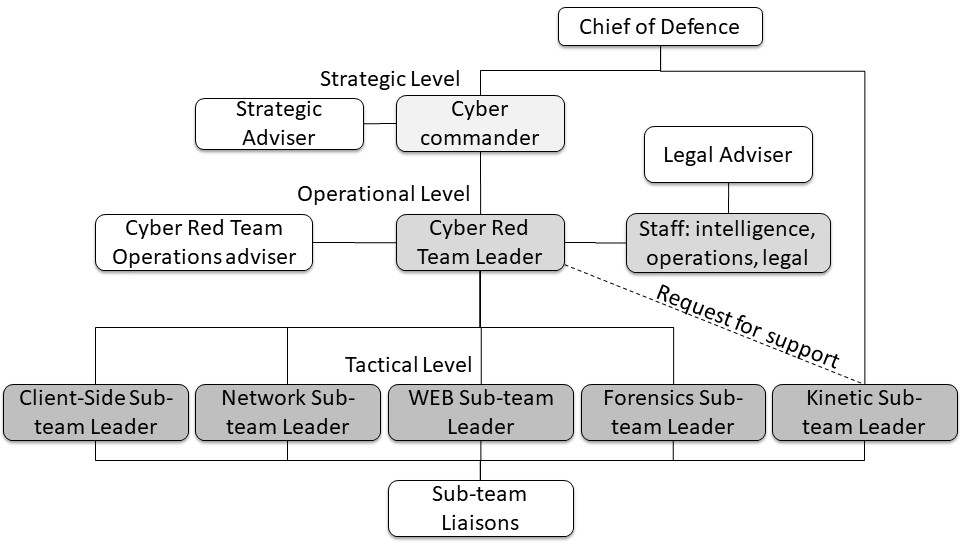
\includegraphics[width=1.0\textwidth]{./img/rt-org.jpg}
    \caption{``Crossed Swords 2019'' cyber red team chain-of-command}
    \label{fig:rtorg}
\end{figure}

These teams are subdivided into sub-teams according to the specialization and operational management level:
\begin{enumerate}
    \item \textbf{Red Team}: being the largest team of around fifty experts consists of exercise training audience. The chain-of-command and various sub-teams are the following:
    \begin{enumerate}
        \item \textit{Cyber commander.} The top-level officer in charge of commanding the cyber operation at a political level. This position is offered to the commanders of the NATO member nation cyber commands. Cyber commander, as part of the training audience, manages and coordinates the cyber operation to reach the set mission goals and coordinates the high-level activities, based on the desired effects, of the sub-teams. Even if the role of the exercise cyber commander might be underestimated it serves as a learning opportunity to the commander on how such cyber-kinetic team would be managed, how to coordinate the activities whilst maintaining the situational awareness. Additionally, this serves an experience for the technical cyber-kinetic team members to always have a clear understanding of the higher commander intentions, provide the situational reports in an understandable manner, and suggest course-of-action options for the mission objective accomplishment;
        \item \textit{Strategic adviser.} Is a member of the exercise development and management team (WT) with the role to provide the advice to the cyber commander, and, if needed, give minor hints to keep the red team activities on the course of designed scenario, as much as it is possible. This option allows exercise developers to explore the nuances and alternative paths for the developed scenario, allowing deviations as long as the end result objectives are met;
        \item {Red team leader group.} This small group of experts, operating at a strategic level and under direct command of the cyber commander, are responsible for fulfilling assigned operational effects by working with the sub-team leaders and ensuring that objectives, force protection, and intelligence activities are correctly executed and reached. This group consists of three experts: the overall red team leader, \gls{opsec} officer, and an intelligence officer;
        \item \textit{Sub-team leaders.} The main red team consists of five expert-focused sub-teams, at a tactical level, which are represented by their leaders. The purpose of every sub-team, consisting of up to ten experts, is to deliver the intended effects at their responsibility area by performing covert infrastructure maintenance, asset protection, stealthy attacks, infiltration of adversary's information systems, precision take-downs, information extraction and gathering, adversary assessment, and cyber-kinetic engagements. Over the exercise iterations it has been identified, that the most applicable size, ensuring its management and providing required capability, of the sub-team is from six to ten experts.
        The role and purpose of every sub-team is as follows:
        \begin{enumerate}
            \item \textit{Client-side attack sub-team.} This team focuses on executing attacks targeted at exploiting end-user (i.e., human vulnerabilities) to get the initial foothold, such as, creating a \textit{spear-phishing} campaign, setting up \textit{watering-hole} or \textit{drive-by} attacks. Once initial breach has succeeded this team performs privilege escalation by exploiting the vulnerabilities on the target client operating system (e.g., MS Windows, GNU/Linux), perform MS Windows domain take-over, conduct lateral movement, control critical processes, such as, unmanned aerial or ground vehicle management graphical user interface, and ensure persistence in the target computer network;
            \item \textit{Network attack and exploit development sub-team.} The goal for this team is to target exposed computer network services, gain control over them by abusing the misconfiguration, poor implementation, abuse, or developing and exploiting software vulnerabilities. Additionally, this team is conducting IP network (IPv4 and IPv6) and service mapping, and executing attacks against specialized systems, such as, tactical radio networks, mobile operator base stations, and \gls{ics} elements;
            \item \textit{Web-application attack sub-team.} For this team all web-based systems and technologies, such as, web-applications, services, and back-end relational databases, are the target. This team extracts valuable information from the web-applications, such as, user credentials, e-mails, or application source code, as well as breaches the security of an exposed web-application to gain access to the internal network services, and establish persistence;
            \item \textit{Digital battle-field forensics sub-team.} The main effort of this team is to perform data carving and artefact extraction from various sources, such as, hardware devices (e.g., smart phones, portable computers and other electronics), computer memory or hard disk images, by applying digital forensics techniques. This team uniquely serves as the bridge between the cyber and kinetic operational components as it is tasked to perform analysis of forensic evidence extracted either by the cyber sub-teams or brought in from the field by the kinetic team. The goal of the forensic team is to extract valuable evidence or information, such as, intelligence information, sensitive documents, malware command and control server addresses, passwords, or enemy communication channel encryption keys; and
            \item \textit{Kinetic forces sub-team.} This team formed from trained military and law-enforcement experts performing various kinetic operations, such as, forced entry, covert access, hardware extraction, target capture or take-down, intelligence collection, surveillance, or kinetic activities on enemy territory. The interaction between the red team provides the one of the key aspects for cyber-kinetic game-play and operation execution. This team is managed and trained by industry experts (e.g., HTCI -- High-Tech Crime Institute) and \gls{sof} instructors. The created scenario is designed to have the interdependencies within the red team and anticipates the cyber-kinetic cooperation. For example, the cyber red team might identify a lead, by collecting and assessing the digital evidence, to a crucial asset, such as, air-gapped server containing adversary communication encryption keys, which is not directly reachable by cyber means and requests the kinetic force engagement for planning and executing the operation to acquire it. In this example, the kinetic force is trained to identify needed hardware, learn its extraction techniques, and preserve digital evidence. Also the kinetic force team might depend on cyber team's support, for example, when executing a forced entry into adversary's data centre protected by a blast-door this can be either can be achieved either by kinetic attack (e.g., use of explosives or physical force) or by cyber means (e.g., targeting the ICS/SCADA system controlling the doors or cutting the power to trigger fail-safe procedures). In this example, depending on the entry method, the kinetic force team might have less or more time to perform the intended activities.
        \end{enumerate}
        \item \textit{Sub-team liaisons.} For every mentioned sub-team there is an attached WT liaison responsible for observing and, if required, providing minor hints to the sub-team leader to ensure that the team is not wasting too much time on some targets, such as, cyber decoys and honeypots, and does not deviate from the intended scenario too much; and
        \item \textit{legal advisers.} With advisers embedded to assist every level -- political, strategic, and tactical. The role of these experts is to provide their assessment of the activities form the international and domestic law perspectives. They are not allowed to break the game by denying certain actions, but more giving an insight to the participants on legal implications and consequences of their activities. These experts are heavily used by the training audience to verify and confirm the legality of their planned actions and choose the one compliant or with least consequences. This gives not only the experience and comprehension of ramifications for various taken activities to the technical members of the red team, but also the training experience to the legal advisers as they have to tackle the questions and situation which they might not encounter on day-to-day basis.
    \end{enumerate}
    \item \textit{Blue Team.} Is a small team of up to four experts experienced in conducting cyber red team activities. This team is under direct control and supervision by the white team and is used to manage the cyber red team's progression within the adversary's computer networks. The main tasks for this team are user and adversary simulation. As a user simulation role-player, they are directly engaged in client-side conducted activities, such as, examining and deciding to open received malicious attachments, visiting the web links, or browsing the in-game web services. With this role their task is to observe, assess and deny or permit the cyber red team's initial foothold, based on the quality and delivery method sophistication level. As an adversary simulation team, their task is to detect the cyber red team's presence, related \gls{ioc}, assess the scale, sophistication and red team objectives, and, if permitted, compromise the red team operational infrastructure in a counter-red team operation. By adjusting the level of the resistance of the adversary's information system the cyber red team will have to take this into account when executing their attacks, maintaining \gls{opsec}, and protecting their assets;
    \item \textit{White Team.} Is a small group of experts, typically no more than two, responsible for controlling and steering the exercise according to the developed scenario. As mentioned before, deviations from scenario are accepted and some-times encouraged, as long as, the overall focus is not lost, and mission objectives can be reached. It has to be noted, that the exercise does not have the ultimate goal of succeeding in accomplishing the intended scenario and fulfilling entirely the laid mission goals by any means necessary. Depending on the activities pursued by the red team, their course-of-action and time limitations, the mission might be a failure, as it can happen in real life. Within the past iterations of the exercise the red team only once successfully accomplished all of the laid mission objectives, and in other cases completing them partially.
    \item \textit{Yellow Team.} This team, composed of experts, focuses various areas of threat and anomaly detection, such as, monitoring, big data analytics, intrusion detection, and situational awareness. The tasks and produced results of this team are described in more detail in chapter \ref{sec:feedback}. The most crucial task for this team is to provide the near-real time situational awareness picture to the red team, which represents how the red team operation looks, the detected tools, made mistakes, and identified \gls{tttp}. This fed-back allows the cyber red team to immediately spot the made mistakes and adjust their operations and tool usage to avoid the detection, therefore not only increasing the level of stealth, but also having a better understanding on the used tools and performed actions; and
    \item \textit{Green Team.} Is responsible for tasks, such as, maintaining the cyber range platform, supporting the game network technical requirements, developing the game network hosts and targets, and integrating new technologies either virtual or physical. The game network and introduced technologies are explained in more depth in chapter \ref{sec:scenario}.
\end{enumerate}

The described full-spectrum cyber operation execution, tasking, and command structure represents the technical and human environment with its various interdependencies and nuances, where the current work from the listed publications has been implemented and assessed. This includes:
\begin{enumerate}
    \item Red team -- uses the proposed \gls{tttp}, if they are applicable for a particular objective or to deliver the desired effect. Gaining initial access by developing a custom exploit or fuzzing a proprietary network protocol (\ref{pub:secondPub}) has been successfully executed by the cyber red team against the developed in-game target systems, such as, finding a vulnerable command in a designed network service, allowing stack-based memory buffer overflow exploitation and target system take-over. Established initial foothold on a dual-stack host allows the \gls{cnc} channel establishment back to the red team's operational infrastructure attacking hosts, for specific tasks, such as, covert information exfiltration or individual high-value target system control the custom covert channels have been successfully established (\ref{pub:firstPub}). In addition to these tools, the red team extensively uses also third-party collaboration and post exploitation frameworks (e.g., Cobalt-Strike, Empire, Pupy), which rely on traditional protocols used for \gls{cnc} communications, such as, HTTP, DNS, and SMB. However, when compared to the proposed \textit{nc64} capabilities, these typical channels are relatively easily detected by the yellow team, and the red team has to make sure, that they are properly configured and adjusted to minimize their detection. For such channels, for example, the compliance with expected protocol payloads have to be ensured not to be easily distinguished from the overall traffic, the beaconing (i.e., call-back) timing and randomization has to be considered to avoid behaviour pattern-based matching and used \gls{cnc} protocols have to make sense for the target hosts. The \gls{ics} oriented zero-day development (\ref{pub:thirdPub}) has been implemented in the game environment, and the red team is faced with identifying weaknesses and exploiting them. All of the described attack vectors in that publication have been successfully also transferred into the exercise and cyber red team has developed the exploits under supervision of an instructor. Due to exercise time restrictions, the instructor gives some leading hints in form of a question allowing the training audience to understand and successfully accomplish the goal within a reasonable time frame. For example, the PROFINET IO attack has been used to control the adversary's data centre bunker doors, and IEC-104 and Martem RTU attacks -- to disable the enemy's military base power supply;
    \item Adversary simulation team (BT) -- it is not mandatory for this team to use any of the proposed cyber-red team oriented \gls{tttp}, as for the adversary simulation team it is not the main purpose of remaining undetected. In some cases, the techniques and tools as described in \ref{pub:secondPub} have been used against the cyber red team's operational infrastructure, but in most cases the red team \gls{opsec} failures are used against themselves, such as, unchanged default passwords on the attacking machines, not removed metadata in the delivered infected documents, or leaving unattended back-doors;
    \item Legal advisers -- according to the scenario, as introduced in the following chapter \ref{sec:scenario}, the artificial conflict tackles both international and domestic law. In cases, when international law applies, the work in \ref{pub:eighthPub} is used to consult the situation and assess its legal implications;
    \item Yellow team -- to provide the near real-time feedback and situational awareness picture, as described in detail in chapter \ref{sec:feedback}, the solutions for Syslog data aggregation, parsing and correlation (\ref{pub:fourthPub}, \ref{pub:fifthPub}) are used alongside with the other technologies allowing threat detection and visualization. The cyber red team has to be trained to identify the cyber deceptions and honey-pots (\ref{pub:sixthPub}), therefore a set of various honey-pots (e.g., low- and high-interaction, and adaptive) and decoys with planted \textit{breadcrumbs} are placed within the adversary's computer networks. This serves not only as a method to represent the situational awareness to the red team but attempts to teach the experts that not all systems have to be targeted and how to identify the decoys. The \textit{Frankenstack} framework (\ref{pub:seventhPub}), consisting of multiple interconnected tools and solutions, is the core solution developed by the yellow team to provide near real-time situational awareness to the cyber red team; and
    \item Green Team -- to make the exercise challenging, technically interesting and represent real-life systems as much as possible, the research results (\ref{pub:thirdPub}) are adapted and re-implemented from real cyber operations. The goal for such system integration is to give opportunity to the red team to practice attacks against real systems, which are not available to the participants on day-to-day basis. The introduced technical challenges are covered in more detail in the upcoming chapter \ref{sec:scenario}.
\end{enumerate}

\subsection{Technical Environment, Exercise scenario and Legal Considerations}
\label{sec:scenario}
\textbf{Technical environment and scenario.}
The ``Crossed Swords'' (XS) exercise game network is hosted on a cyber range running VMware ESXi hypervisor and it consists of around 200 virtual machines for in-game core networking, simulated Internet, cyber red team segment, and a set of target networks. Not all intended technical game-play elements can be virtualized, therefore the game network is expanded by connecting physical hosts and systems through the cyber range infrastructure. Before creating the overarching geo-political scenario, the technical scenario is established based on the core development team ideas and intended technical game-play intentions.
Due to XS being relatively small, with respect to the game-network scale and training audience size, experimentation and introduction of new, recently prototyped, and orthodox technologies can be afforded making the technical game-play more attractive and as close to the real-life as possible. The network also uses the traditional \gls{it} systems to provide the networking and common workstation operating systems, such as, MS Windows and GNU/Linux, to provide replicate the structure of a regular office and business networks.
The following list briefly summarizes some of the technologies introduced in the XS game series, to highlight the technical level:
\begin{enumerate}
    \item Bunker door -- a system, running a set of interconnected Siemens developed S7-1200 \gls{plc} based PROFINET IO-devices, is controlling the bunker door. The cyber red team has to analyse and reverse-engineer the PROFINET IO RT protocol to inject remotely the commands to open or close the bunker door;
    \item Alarm system -- a bunker door is protected by the Paradox supplied alarm system and, before the door can be opened, the alarm system has to be targeted remotely by analysing the used bus-protocol, and capturing and decoding the PIN code;
    \item CCTV IP camera -- attack implies the cyber red team finding and exploiting the flaws in the actual IP-based surveillance camera web interface to gain full control remotely;
    \item Distributed power-grid -- a system based on IEC-61850 and IEC-60870-5-104 industrial Ethernet protocol series and a Martem produced \gls{rtu} is used to manage and supervise the distributed power-grid. The red team has to reverse-engineer the IEC-104 protocol and perform remote command injection to control the power supply either by turning it off or on;
    \item Anonymization network -- red team has to infiltrate the real \textit{i2p} anonymization network to intercept and modify the \gls{cnc} communication channel running over that network;
    \item Unmanned aerial vehicle (UAV) -- adversary's Threod manufactured UAVs, flying over or approaching the protected territory, have to targeted to gain control over the provided video stream, taking over the steering, or destroying the UAVs;
    \item Unmanned ground vehicle (UGV) -- Milrem developed UGVs serve as an adversary-controlled tank force and the cyber red team is tasked to take full control over them by targeting either the used network protocols or the controlling workstation;
    \item Maritime navigation -- a vessel's steering and tracking system based on the OTH-GOLD (Over-The-Horizon GOLD) and AIS (Automatic Identification System) maritime protocols is targeted by the red team to gain control over the ship and inject naval tracks to confuse the situational awareness;
    \item Radio communication network -- the network based on Harris constructed military-grade radio stations has to be infiltrated by the red team via extracting the encryption keys for the communications running over the radio carrier;
    \item Mobile network base stations -- the cyber red team has to infiltrate the LMT (Latvian Mobile Telephone) operator provided base stations connected to the actual mobile network, analyse and parse the intercepted communications to decode the adversary agent's message exchange (SMS) and pinpoint their physical location;
    \item Mobile 4G network -- red team is tasked to gain access to the Ericsson developed 4G mobile network equipment and execute further attacks against connected nodes;
    \item Railroad control station -- a system based on Siemens created S7-1200 \gls{plc}, running s7comm+ protocol, is used to control the in-game railroad network. The red team is tasked to gain control over the railroad control stations either to stop or derail the train; and
    \item Environment monitoring wireless sensors -- the red team has to control the Defendec provided Smartdec wireless sensors to track the physical location of an adversary troops.
\end{enumerate}

The various technical challenges implemented across nearly all of the game-net systems, are designed in a way, that no single sub-team of the red team can solve them on its own. To achieve this, cooperation, information exchange, objective tracking, and operation management is emphasized to provide the collaborative training experience and attempting to push the participants out of their comfort zones. The technical scenario, being time limited and fast-paced, cannot be fully solved, therefore the cyber red team has to consider ways and approaches on how to prioritize the technical objectives and manage the focus of force to accomplish the overall mission objectives within the exercise time.

The integration of real-life vulnerabilities and systems, such as, the ones as described in \ref{pub:thirdPub}, deliver the learning perspective to the exercise participants. Examining, developing exploits, and attacking the systems which are widely used for automation and industrial process control are challenging and allow the training audience to comprehend the actual state of security for such industrial components. Furthermore, some participants might have such systems in their organizations, but are not allowed to executed attacks or tests due to them being in a production state.
Cyber red team members, with some guidance by the instructors, follow the full weakness identification, vulnerability determination, and exploit development life-cycle as described in the chapter \ref{sec:impact}. Such approach has allowed the participants to successfully exploit the industrial control protocols and devices (\ref{pub:thirdPub}).

\textbf{Exercise scenario.}
The technical scenario, describing the interdependencies, attack vectors, and alternative paths, only covers the part for the actual work to be conducted by the exercise participants. To deliver the context, reasoning, and clear objectives, the overarching scenario is required. This scenario provides the elements, such as, the state-of-the-world background, geo-political situation, intelligence information on what has happened, what is the impact suffered, why the response is being triggered, what are the objectives and rules of engagement.
The main geo-political story revolves around a fictitious group of Cyberbian islands, where every island is a country with its technological advancements, political stance, alliances, and intentions. The three island-countries are Berylia, Crimsonia, and Revalia. Berylia being the smallest with a modest military force, part of NATO alliance, and its main economic income originating from the electronics manufacturing. Crimsonia is the largest island with a strong military, rich in natural resources, not part of any alliance, and is expressing some signs of aggression against its neighbouring island-countries. Revalia is a small, self-sustained, and politically neutral country. Within the scenario, the exercise participants assume the role of Berylian rapid response team, which is assembled to address the looming crisis, maintain the resiliency of the national critical information infrastructure, and accomplish the mission goals.
Every year, with a new exercise edition, the scenario evolves and the tensions between Berylia and Crimsonia have been escalating, ranging from Crimsonia conducting a series of debilitating cyber attacks against Berylian \gls{cii}, abuse of a neutral nation infrastructure for operation conduct, placing insiders and double-agents, forming military blockades, up to launching a military invasion of Berylia. The various levels of conflict are designed to explore the technical, cyber-kinetic, and legal game-plays as every particular state opens new opportunities and provides flexibility in conducting the responsive computer network operations. The operational environment for the kinetic force's unit is extremely important, as this restricts, or enables, some types of activities to be exercised.

\textbf{Legal considerations.}
A part of the exercise scenario consists of legal game-play. Despite the exercise not having legal aspects as the primary objectives, the legal guidance and considerations are incorporated in the form of legal scenario injects aimed to trigger the discussion and legal implication consideration during the situational report meetings. Legal advisers are assigned to every level of the chain-of-command to assess and consult the exercise participants. 
The legal aspects of the conducted cyber-kinetic operations and applied \gls{tttp}, within the context of the scenario, tackle at least the following legal considerations as covered in \ref{pub:eighthPub}:
\begin{enumerate}
    \item \textit{Applicable law (Part II)}.
    Depending on the circumstances ruling at the time, the lawyers are tasked to ascertain which regimes of public international law apply to the cyber operations occurring during the exercise. The cyber attack campaigns of the exercise range from those occurring in peacetime to those endangering national and international security. The storyline generally avoids situations of armed conflict. The exercise scenario attempts to bring all of the five operational domains (i.e., land, sea, air, space, and cyber) into the game-play, extended by espionage, and cyber-kinetic operations. Such activities may be addressed by the international human rights law, diplomatic and consular law, law of the sea, air law, space law, and international telecommunications law;
    \item \textit{States entitled to take countermeasures (Rule 24)}. Only state affiliated institutions and organizations, such as, military or intelligence, can conduct responsive activities on the state's behalf as long as the activities they engage in do not constitute an internationally wrongful act. The cyber operations by private entities, such as, business companies or non-governmental organizations (NGO), can never constitute countermeasures in the legal sense. Therefore, the players assume the role of a rapid response team, assembled  on the order of Berylian government, which is placed under the supervision of the military command;
    \item \textit{Effect of \gls{rcd} on third parties (Rule 25)}. Due to the fact that \gls{rcd} has extraterritorial nature and implicates pursuing the adversary, as well as, performing malicious service take-down within the cyberspace, the legal advisers are required to assess the legality of the \gls{rcd} effects on the third parties. These activities may include operations, such as, third-party \gls{vps} take-over, hacking adversary controlled \gls{cnc} servers on the Internet, back-dooring or re-weaponizing the malicious code used by the adversary and compromising public web services to plant the targeted exploit-kits. Since such operations are intentional, both from the adversary and defender side, they have an effect on third-party owned systems or against ones residing in a neutral state (i.e., Revalia). For the red team to complete their mission objectives, the \gls{rcd} activities have to be deemed lawful, the various possible paths have to be explored, their effects evaluated, and necessary precautions taken, if such are reasonably possible;
    \item \textit{Limitations on \gls{rcd} (Rules 23, 26, 72, 73, 113)}. Depending on the legal qualification of the \gls{rcd} operations, various limitations, such as, concerning necessity, proportionality, imminence and immediacy, are attached to this operation. The legal advisers are tasked to identify any applicable limitations, such as, requirements for the \gls{rcd} to be necessary and proportionate, and provide these legal implications to the commander or sub-team leaders. The scenario addresses both the cyber and kinetic attacks and activities performed by the adversary against the defended state and its \gls{cii}. Those include malicious operations, such as, serious cyber attacks, espionage, sabotage, and deployment of malware (e.g., condition-activated logic-bombs) with the goal to debilitate the state's critical services and capabilities. Adversary's kinetic activities include operations, such as, armed drone attacks, navy blockades, placement of a large amount of troops on the borders, and expeditionary force deployment. The game-play is initiated by the series of escalating events leading to ongoing or imminent threat, which may serve to prove the necessity of the taken responsive operations, which are evaluated by their proportionality and delivered effect.
    As derived from the scenario, the defending state has to immediately respond to an ongoing or imminent threat to ensure the resiliency and protection of critical assets relevant to the security, functionality and well-being of the state;
    \item \textit{Self-defence against an armed attack (Rule 71)}. The scenario is designed in such a manner that the severity offensive action against the victim state amounts to to an armed attack, thus permitting to respond in self-defence with an immediate asymmetric responsive cyber operations against a stronger and advanced adversary. The scenario can be designed more subtle and with less tensions, however, in such case the training audience would struggle proving the necessity to pursue the adversary and infiltrate their network, which would have an impact on the overall game-play and achieving the currently set mission and training objectives;
    \item \textit{Geographical limitations of cyber operations (Rule 81)}. The effects of a cyber operations have to be limited to the intended target information systems and geographical locations. This, although not always being possible to limit geographically, is taken into consideration by the red team when executing the cyber operation which may include the activities, such as, placement of drive-by exploit-kits on third-party services. The red team might not be aware of geographical location of a targeted asset in cyberspace, however, when such attack campaign is executed, measures are taken to restrict its spread within the intended target's network address ranges if it is possible;
    \item \textit{Means and methods of cyber warfare (Part IV, Chapter 17, Section 5)}. The exercise scenario plays on the various levels of aggression and conflicts without entering the state of war. Despite cyber warfare not being applicable directly it is still to be considered and applicable methods have to be evaluated accordingly, since, within the played-out high-tension scenario, it could unexpectedly escalate to an armed conflict and the state of war;
    \item \textit{Precautions (Part IV, Chapter 17, Section 7)}. For the executed cyber operations, the red team is asked to exercise constant care, perform verification of targets, choice of means or methods, choice of targets, evaluate proportionality, and estimate the effects of cyber attack whenever it is reasonably possible and applicable;
    \item \textit{Cyber operations in neutral territory (Rule 151)}. The adversary may proxy their cyber attacks or route the kinetic attack, such as, drone flying through neutral state's air space before heading to the intended target. In such cases, the red team's response might have uncertainty and limitations on taken actions in the neutral state's cyberspace. The red team might be tasked with pursuing alternative paths or collecting more attribution evidence, before executing cyber operations within the targets in neutral state's cyberspace; and
    \item \textit{False-flag and no-flag operations.} For the red team to protect their identity, assets and intended objectives, a false-flag or no-flag operation would be considered to be executed to imply uncertainty and make attribution harder. From the technical perspective, the cyber red team might adapt the known \gls{tttp} of a chosen threat actor to deceive the adversary. From the legal point of view, it is not clear if such operations are permitted when, for example, impersonating and adversarial profile of a threat actor with high certainty attributable to a third state.
\end{enumerate}


\subsection{Training Assessment and Real-time Feedback}
\label{sec:feedback}
One of the key aspects of the ``Crossed Swords'' exercise is to provide the environment, where the cyber red team can experiment, practice applicable \gls{tttp} and observe their effects in near real-time. Such opportunity provides the necessary feedback to the exercise participants for their tool and procedure stealthiness and efficiency, as well as, to the exercise management to evaluate the progress of the red team and the fulfilment of training objectives.
To accomplish this, a dedicated framework, called the \textit{Frankenstack} and described in \ref{pub:seventhPub}, is developed to deliver the required visibility through meaningful visual means and notifications.

The \textit{Frankenstack} development is facilitated and coordinated by NATO CCD CoE since 2016, with a group of an international team of experts. The development team is assembled from technical experts in the field of monitoring, data visualization, threat detection and assessment, and big data analytics. The contributions include NATO CCD CoE partners, such as, Arc4dia, Stamus Networks (Suricata IDS), Greycortex, Cymmetria, Tallinn University of Technology, CERT.LV, and CERT-EE.
The \textit{Frankencoding} events\footnote{Frankencoding. \url{https://github.com/ccdcoe/Frankencoding}. Accessed: 23/11/2018} have resulted in an ongoing \textit{Frankenstack} development with its source code released publicly\footnote{Frankenstack. \url{https://github.com/ccdcoe/frankenstack}. Accessed: 23/11/2018} on GitHub under the MIT license.

\textbf{Goals and design principles.}
The operational principles of the developed framework are defined as follows:
\begin{enumerate}
    \item \textit{increase stealthiness} of the red team executed operation, by providing comprehensive and real-time situational picture;
    \item \textit{improve \gls{rt} coordination} through granular multi-layered view of the detected attacks;
    \item \textit{analyse \gls{tttp}} and allow the red team to identify the weaknesses and improve the operational performance;
    \item \textit{open-source} tool usage as the building blocks for the \textit{Frankenstack} to lower the needed costs and increase the framework maintainability;
    \item \textit{customizable} and interchangeable open-source modules to be replaced for more efficient operations or introduced to expand the existing functionality;
    \item \textit{high automation} demands to minimize the latency introduced by human-in-the-loop, by applying solutions, such as, data clustering and pattern mining algorithms;
    \item \textit{real-time} provision of the identified threats to allow the adjustment of the red team campaign in a timely manner;
    \item \textit{transparency and visibility of actions} delivering the processed information for further analysis at different levels, such as, host-based, or network-based, to the red team members;
    \item \textit{adequately detailed} information to be provided to the red team not experienced in system monitoring or data analysis, while still providing enough detail in line with the current game-play progress of the red team; and
    \item \textit{correlated attack visualisation} to make the detected attacks and threats easily understandable to the exercise participants, exercise control, and observers. This has been implemented by a novel web-based Event Visualization Environment (EVE) and displaying the detected attacks on an interactive network map.
\end{enumerate}

\textbf{Integration in the game network.}
The solution is easily deployable in the game network and can accept any possible sources of information to be further processed, which can be from at least the following origins:
\begin{enumerate}
    \item \textit{ERSPAN (Encapsulated Remote Switched Port ANalyser)} traffic mirror collecting all the network data recording, parsing, and deep packet inspection;
    \item \textit{NetFlow} from game network routers for traffic statistical analysis and evaluation;
    \item \textit{data from the systems}, such as, system performance metrics (e.g., CPU load, HDD utilization, network interface card statistics), and logs (e.g., Syslog, and application textual log-files);
    \item \textit{honeypots and cyber decoys} placed in the network to attract and deceive the cyber red team into revealing its \gls{tttp}; and
    \item \textit{aggregates the information from all sources} in textual format allowing this to be reduced to a log correlation and analysis problem.
\end{enumerate}

\textbf{Assessment.}
During the ``Crossed Swords 2017'' execution the members of the white team performed the assessment of the deployed \textit{Frankenstack} solution for its usefulness and training benefits. The identified findings were addressed and incorporated into the following exercise editions. The conducted expert qualitative interviews and online survey results reflected the following:
\begin{enumerate}
    \item the deployed tools themselves do not increase the learning perspective, but is up to how red team members perceive and use the tools;
    \item the addition of situational awareness solutions to the exercise is welcome and seen as a necessary component;
    \item the four large screens in the execution room, showing the yellow team provided information, was preferred and checked approximately every 45 minutes by the majority of the training audience;
    \item exercise participants also used the opportunity to access the \textit{Frankenstack} dashboards locally on their computers and dig deeper when attempting new attack vectors;
    \item \textit{Alerta} tool, showing the identified attacks as priority categorized alerts, was found most useful by the majority of the trainees;
    \item it was acknowledged, that ease of use should be further improved especially when considering the merger of high intensity technical exercise with monitoring tools not known to all participants;
    \item majority of the training audience strongly agreed that the provided situational awareness was beneficial to the learning process, was accurate and delivered in acceptable speed;
    \item the larger part of the training audience agreed that they learned more regarding how their actions can be detected and tried to be stealthier; and
    \item integration of various tools into the \textit{Frankenstack} has to be evaluated carefully to avoid visual distractions and making the output more self-explanatory.
\end{enumerate}

\subsection{Chapter Conclusions}
The technical exercise ``Crossed Swords'', created and led by the author, integrates all of the research from the listed publications to deliver the innovative and novel training environment for the cyber red team. The flexibility and agility of the exercise permits it to be used as a platform for experimentation, research, and verification of new ideas and concepts. By exploring yet not fully understood concepts of cyber red team assembly and structure, cyber operation management and execution, \gls{tttp} applicability and stealth, near real-time feedback, and intense game-play scenario, permits to identify and verify the functional aspects of cyber operation nuances, which can be integrated into actual cyber operation execution.
The exercise strives to provide to the training audience the increased and recognized training experience and benefits by combining the technical, operation management, and legal aspects. The conducted survey (see appendix on page \ref{app:survey}), with an intention to gather overall feedback and impressions from the exercise participants since year 2014, identifies the learning benefits acknowledged by the training audience.
The unique near real-time feedback, delivered to the cyber red team via the \textit{Frankenstack}, permits the team members to assess and increase their skills, employed techniques and tools, adapted tactics and procedures, and promotes deeper understanding of the situational awareness and cyber red team executed responsive computer network operation.
